\documentclass[a4paper,12pt]{article}
\usepackage[utf8]{inputenc}
\usepackage{amsmath}
\usepackage{graphicx}
\usepackage{float}
\usepackage{svg}
\usepackage{hyperref}
\usepackage{minted}  
\usepackage{titlesec}

\setcounter{section}{-1}

\title{You Only Look Once (Yolo)}
\author{BEX Roméo, RIVALDI Tristan, LAMURE Maxence}
\date{24 Septembre 2024}

\begin{document}

\maketitle

\tableofcontents

\newpage

\section{Introduction}

La détection d'objets est une tâche cruciale en vision par ordinateur, utilisée dans des domaines comme la conduite autonome, la surveillance et les systèmes de sécurité. Elle nécessite non seulement la localisation des objets dans une image, mais aussi leur classification, tout en garantissant un temps de traitement rapide pour les applications en temps réel.

L'approche YOLO (You Only Look Once) révolutionne la détection d'objets en traitant cette tâche comme un problème de régression unique, passant directement de l'image complète aux prédictions des boîtes englobantes et des classes d'objets. Cette méthode permet d'atteindre des vitesses élevées, jusqu'à 45 images par seconde, ce qui est idéal pour les systèmes en temps réel. Cependant, YOLO présente certaines limites, notamment dans la précision de la détection des petits objets.

Ce rapport explore l'architecture de YOLO, ses fondements mathématiques, ses performances par rapport aux autres méthodes de détection, ainsi que ses avantages, inconvénients, et applications concrètes.

\section{Système de détection Yolo}

\begin{figure}[H]
    \centering
    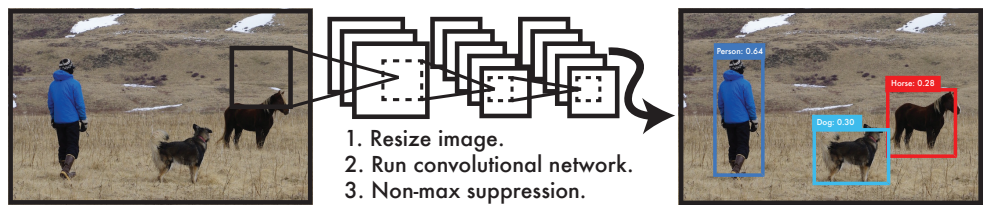
\includegraphics[width=0.9\linewidth]{illustration-yolo.png}
    \caption{Système de détection Yolo}
    \label{fig:enter-label}
\end{figure}

Comme on peut voir ci-dessus, la reconnaissance d'image est divisée en 3 parties qui sont :    
- La première étape consiste à faire un \textbf{redimensionnement} de l'image d'entrée à une taille fixe de 448 × 448 pixels. Cela permet d'uniformiser la taille des images, peu importe leurs dimensions d'origine, ce qui facilite le traitement par le réseau de neurones.

- Ensuite, l'image redimensionnée est passée dans un \textbf{réseau de neurones convolutionnel (CNN)}. Le CNN traite l'image pour extraire des caractéristiques et prédire plusieurs boîtes englobantes (bounding boxes) et les classes d'objets correspondantes. Le réseau prédit simultanément plusieurs objets dans l'image.

- Après que le modèle a généré les prédictions, la dernière étape est \textbf{la suppression non-maximale}. Cette méthode élimine les boîtes englobantes qui se chevauchent et qui représentent le même objet, en ne gardant que la boîte avec le score de confiance le plus élevé. Cela permet d'éviter les multiples détections d'un même objet.


\section{Fonctionnement du réseau de neurone}

Le réseau de neurones YOLO est une architecture de réseau convolutionnel profond (CNN) qui convertit une image en entrée en une série de prédictions de boîtes englobantes et de classes d'objets. Contrairement aux approches traditionnelles, YOLO traite la détection d'objets comme un \textbf{problème de régression} global et non comme un ensemble de sous-tâches indépendantes (comme la génération de régions et la classification).

\subsection{Prétraitement de l'image d'entrée}
La première étape du fonctionnement de YOLO est le \textbf{redimensionnement de l'image d'entrée} à une taille fixe de \(448 \times 448\) pixels. Cette étape permet de standardiser la taille des images avant de les passer dans le réseau.

\subsection{Extraction des caractéristiques avec les couches convolutionnelles}

Les \textbf{couches convolutionnelles} sont responsables de l'extraction des \textbf{caractéristiques} importantes de l'image d'entrée. Les caractéristiques extraites sont utilisées pour détecter des objets à différentes échelles dans l'image.

\subsubsection{Convolution}
Chaque couche convolutionnelle applique un ensemble de \textbf{filtres} à l'image d'entrée pour extraire des caractéristiques locales. Mathématiquement, une convolution est l'opération suivante :
\[
h_{ij}^{(k)} = (W^{(k)} * x)_{ij} = \sum_m \sum_n W_{mn}^{(k)} x_{(i+m)(j+n)}
\]
Où :
\begin{itemize}
    \item \( h_{ij}^{(k)} \) est la valeur du pixel \( (i, j) \) dans la \textbf{carte de caractéristiques} résultante de la convolution avec le filtre \( k \),
    \item \( W^{(k)} \) est le \textbf{noyau} (ou filtre) de convolution \( k \),
    \item \( x \) est l'image d'entrée ou la sortie de la couche précédente,
    \item L’opérateur \( * \) représente la convolution.
\end{itemize}

Cette opération permet au réseau d'apprendre des motifs et des structures (comme des bords ou des coins) présents dans l'image à différentes échelles et positions.

\subsubsection{Activation ReLU}
Après chaque convolution, une fonction d'activation non linéaire est appliquée, en général la fonction \textbf{ReLU (Rectified Linear Unit)} :
\[
\text{ReLU}(z) = \max(0, z)
\]
Cette activation permet de rendre le modèle non linéaire, ce qui est essentiel pour capturer des relations complexes entre les pixels d'entrée.

\subsection{Prédiction des boîtes englobantes et des classes avec les couches entièrement connectées}

Après plusieurs couches convolutionnelles, YOLO utilise des \textbf{couches entièrement connectées} pour transformer les cartes de caractéristiques extraites en \textbf{prédictions concrètes} de boîtes englobantes et de classes. 

L'image est divisée en une grille de taille \( S \times S \), généralement \( S = 7 \). Chaque cellule de la grille est responsable de prédire un certain nombre de \textbf{boîtes englobantes} (bounding boxes) et les \textbf{classes d'objets} pour les objets dont le centre se trouve dans la cellule.

\subsubsection{Prédiction des coordonnées des boîtes englobantes}
Pour chaque cellule de la grille, le réseau prédit les coordonnées \(x\), \(y\), \(w\) et \(h\) des boîtes englobantes :
\begin{itemize}
    \item \( x \) et \( y \) représentent les \textbf{coordonnées du centre} de la boîte, relatives à la cellule (donc comprises entre 0 et 1).
    \item \( w \) et \( h \) représentent la \textbf{largeur} et la \textbf{hauteur} de la boîte, relatives à la taille totale de l'image.
\end{itemize}

Ces prédictions sont normalisées afin que :
\[
0 \leq x, y \leq 1, \quad 0 \leq w, h \leq 1
\]
Les coordonnées sont obtenues à partir des \textbf{cartes de caractéristiques} générées par les couches convolutionnelles. Elles sont multipliées par des poids et additionnées à des biais appris durant l'entraînement.

\subsubsection{Prédiction des scores de confiance}
Chaque boîte englobante est associée à un \textbf{score de confiance} \(C\) :
\[
C = \text{Pr(Object)} \times \text{IoU}_{\text{pred, truth}}
\]
Où :
\begin{itemize}
    \item \( \text{Pr(Object)} \) est la probabilité qu'un objet soit présent dans cette boîte,
    \item \( \text{IoU}_{\text{pred, truth}} \) (Intersection over Union) est une mesure de la qualité de l'ajustement entre la boîte prédite et la boîte réelle. Il permet d'évaluer la similarité entre deux ensembles que sont les Bounding Boxes
\end{itemize}

\subsubsection{Prédiction des classes d'objets}
Pour chaque boîte prédite, le réseau prédit une distribution de probabilités sur les \textbf{classes d'objets} possibles. Ces probabilités sont obtenues à l'aide d'une fonction \textbf{softmax} :
\[
p_i(c) = \frac{e^{z_c}}{\sum_{c' \in C} e^{z_{c'}}}
\]
Où :
\begin{itemize}
    \item \( z_c \) est le score brut (logits) de la classe \(c\),
    \item \( p_i(c) \) est la probabilité que la boîte \(i\) contienne un objet de la classe \(c\).
\end{itemize}

\subsection{Fonction de perte de YOLO}

Le réseau YOLO est entraîné pour minimiser une \textbf{fonction de perte} qui combine trois composantes :
\begin{enumerate}
    \item \textbf{Perte de localisation} : Mesure la différence entre les coordonnées des boîtes prédite et les boîtes réelles (ground truth).
    \[
    \text{Loss}_{\text{loc}} = \lambda_{\text{coord}} \sum_{i=0}^{S^2} \sum_{j=0}^{B} \mathbf{1}_{\text{obj}}^{ij} \left[ (x_i - \hat{x}_i)^2 + (y_i - \hat{y}_i)^2 + \left( \sqrt{w_i} - \sqrt{\hat{w}_i} \right)^2 + \left( \sqrt{h_i} - \sqrt{\hat{h}_i} \right)^2 \right]
    \]
    
    \item \textbf{Perte de confiance} : Compare les scores de confiance prédits et réels.
    \[
    \text{Loss}_{\text{conf}} = \sum_{i=0}^{S^2} \sum_{j=0}^{B} \mathbf{1}_{\text{obj}}^{ij} (C_i - \hat{C}_i)^2 + \lambda_{\text{noobj}} \sum_{i=0}^{S^2} \sum_{j=0}^{B} \mathbf{1}_{\text{noobj}}^{ij} (C_i - \hat{C}_i)^2
    \]
    
    \item \textbf{Perte de classification} : Évalue la différence entre les classes prédite et les vraies classes d'objets.
    \[
    \text{Loss}_{\text{class}} = \sum_{i=0}^{S^2} \mathbf{1}_{\text{obj}}^{i} \sum_{c \in \text{classes}} (p_i(c) - \hat{p}_i(c))^2
    \]
\end{enumerate}

\subsection{Optimisation du réseau}
Pendant l'entraînement, les \textbf{poids} du réseau de neurones sont ajustés pour \textbf{minimiser la fonction de perte} à l'aide d'un algorithme d'optimisation, tel que la \textbf{descente de gradient stochastique} (SGD) ou \textbf{Adam}. 

\section{Résultats, forces et faiblesses}

\begin{figure}[H]
    \centering
    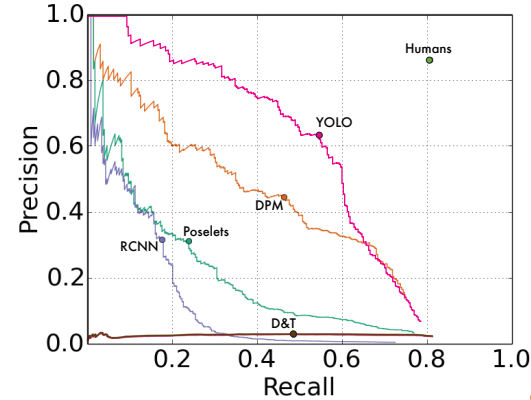
\includegraphics[width=0.8\linewidth]{yolo-recall-precision.png}
    \caption{Enter Caption}
    \label{fig:enter-label}
\end{figure}


En abscisse on peut voir le Racall qui mesure la capacité du modèle à détecter tous les objets pertinents dans une image. Il s'agit du pourcentage des objets réellement présents qui ont été correctement détectés par le modèle. 
En ordonnée la précision qui mesure la proportion de prédictions faites par le modèle qui sont correctes. 
Ansi YOLO se place en premières places au vu de ces différents algorithmes.

\section{Conclusion}

L'algorithme YOLO propose une approche puissante pour la détection d'objets en temps réel. En reformulant la détection comme un problème de régression, YOLO permet de prédire simultanément plusieurs boîtes et classes dans une image, le tout en une seule passe à travers le réseau. La fonction de perte conçue optimise à la fois la localisation des objets, la confiance des prédictions, et la classification.

\end{document} 
